\subsection{Maze}\label{s:testMaze}

\paragraph{Scenario:} The UAS is flying a mission given by (tab. \ref{tab:missionSetupMazeScenario}) in \emph{closed space} constrained by ground from bottom, airspace constraint from top and building from sides. The maneuverable space is \emph{maze-like} with  \emph{hidden goal waypoint}.

There exists a \emph{Obstacle map} with defined \emph{safety} and \emph{body margins}. \emph{Reference trajectories} (direct interconnection of initial position and \emph{goal waypoint}) is going trough \emph{partially known space} with some charted obstacles.

\begin{table}[H]
    \centering
    \begin{tabular}{c|c||c}
        \multicolumn{2}{c||}{Position} & \multirow{2}{*}{$\mathscr{WP}_1$} \\\cline{1-2}
        $[x,y,z]$           & $[\theta,\varpi,\psi]$           & \\\hline\hline
        $[15,15,0]^T $        & $[0^\circ,0^\circ,0^\circ]^T$    & $[15,75,0]^T$        \\ 
    \end{tabular}
    \caption{Mission setup for \emph{Maze} scenario.}
    \label{tab:missionSetupMazeScenario}
\end{table}

\paragraph{Obstacle set:} \emph{Obstacles} are discovered during a flight by \emph{UAS LiDAR} sensor. The \emph{Obstacle set} is defined in (tab. \ref{tab:obstacleSetMaze}). the obstacles are placed in \emph{virtual grid} with \emph{cell size} $10 \times 10 m$. There are following obstacles:

\begin{enumerate}
    \item $5\times$  \emph{Hospital building} - H-shaped, with two open traps, with minimal body margin in range $0.5 - 1m$, with maximal body margin in range $2.2 - 3.1 m$ and variable \emph{safety margin} in range $1-3 m$.
    
    \item $12\times$ \emph{Unusual trap building} - square shaped building with two traps on neighbouring side, with minimal body margin in range $0.3 - 1m$, with maximal body margin in range $2.3 - 3.5 m$ and variable \emph{safety margin} in range $1-4 m$.
    
    \item $6\times$  \emph{Square building} - square shaped building with minimal body margin in range $3-4 m$, with maximal body margin in range $4-5 m$ and variable \emph{safety margin} in range $1-4m$.
    
    \item $7\times$  \emph{U-shaped Trap} - thin walled U shaped trap designed to catch incoming flying objects, with minimal body margin in range $2-4m$, maximal body margin in range $3-5 m$ and various \emph{safety margin} in range $1-2 m$.
\end{enumerate}

The purpose of these \emph{Obstacles} except \emph{Square building} type is to create false positive path diversions. These diversions are designed to take \emph{UAS} into unsolvable situation. \emph{Avoidance} of traps is possible due \emph{Reach set properties}, because many scenarios for avoidance can be evaluated at once.

\begin{table}[H]
    \centering
    \begin{tabular}{c|c|c|c|c|c}
        \multicolumn{2}{c|}{Obstacle} & \multicolumn{3}{c|}{Body Margin} & \multirow{2}{*}{Safety Margin}\\\cline{1-5}
        position & type & min. & max. & avg. &   \\\hline\hline
        multiple (5) & hospital & $[0.5,1]$ & $[2.2,3.1]$ & $[1.5,3]$  & $[1,3]$ \\\hline 
        multiple (12) & unusual  & $[0.3,1]$ & $[2.3,3.5$] & $[2,3]$    & $[1,4]$ \\\hline
        multiple (6) & square   & $[3,4]$   & $[4,5]$     & $[4,5]$    & $[1,4]$ \\\hline
        multiple (7) & trap     & $[2,4]$   & $[3,5]$     & $[2,4]$    & $[1,2]$ \\
     \end{tabular}
    \caption{\emph{Obstacle set} for \emph{Maze} scenario.}
    \label{tab:obstacleSetMaze}
\end{table}

\paragraph{Main Goal:} Demonstrate static obstacle avoidance in closed space navigation. Focus on determinism of \emph{avoidance run}. Demonstrate the possibilities of primitives \emph{right-hand} maze solver incorporated into \emph{Navigation-loop}.

\paragraph{Acceptance Criteria:}
\begin{enumerate}
    \item \emph{Do not break top/bottom boundaries} - the \emph{UAS} Z coordinate should not leave range $-5$ to $5 m$. The boundary break occurs when there is no feasible horizontal path and UAS needs to climb up to resolve situation.
    
    \item{Minimal safety margin distance} $\ge$ $0m$.
    
    \item\emph{Reach hidden goal waypoint} by solving simple maze (tab. \ref{tab:missionSetupMazeScenario}).
\end{enumerate}

\paragraph{Testing Setup:} The \emph{standard test setup} defined in (tab.  \ref{tab:testMovementOrientations}, \ref{tab:testUASBasicParameters}, \ref{tab:testNavigationGridBasic}, \ref{tab:testAvoidanceGridBasic}, \ref{tab:testUASColoring}) is used with following parameter override:

\begin{enumerate}
    \item \emph{Avoidance grid - type} - \emph{ACAS-like} with enabled \emph{Horizontal maneuvers}
\end{enumerate}

\paragraph{Simulation Run:} Notable moments from  the simulation run (fig. \ref{fig:testCaseMazeSolver}) are following:

\begin{enumerate}
    \item \emph{The Maze} consist from heavy constrained turns: $1^{st}$ turn (fig. \ref{fig:mazeFirstTurn}), $2^{nd}$ turn (fig. \ref{fig:mazeSecondTurn}), and $3^{rd}$ turn (fig. \ref{fig:mazeThirdTurn}). The hidden waypoint reach is given by (fig. \ref{fig:mazeWaypointReach}).
        
    \item UAS is constantly in \emph{Emergency Avoidance mode}, because there is always a presence of obstacle,
        
    \item \emph{Navigation path} is located in slim corridor with width only 3-6 meters. Mutual distance of obstacles is 20 meters and combined margins takes 14-17 meters.
        
    \item \emph{Maze scenario} was very close to urban environment in terms of obstacle density and computation complexity.
        
    \item \emph{Avoidance run} computation complexity scaled linearly with count of active obstacles in Field of View.
    
    \item \emph{Hidden Goal Waypoint} have been reached as shown in (fig. \ref{fig:mazeWaypointReach}). This satisfy \emph{reach hidden waypoint} acceptance criterion. 
\end{enumerate}


\begin{figure}[H]
    \centering
    \begin{subfigure}{0.48\textwidth}
    	\centering
        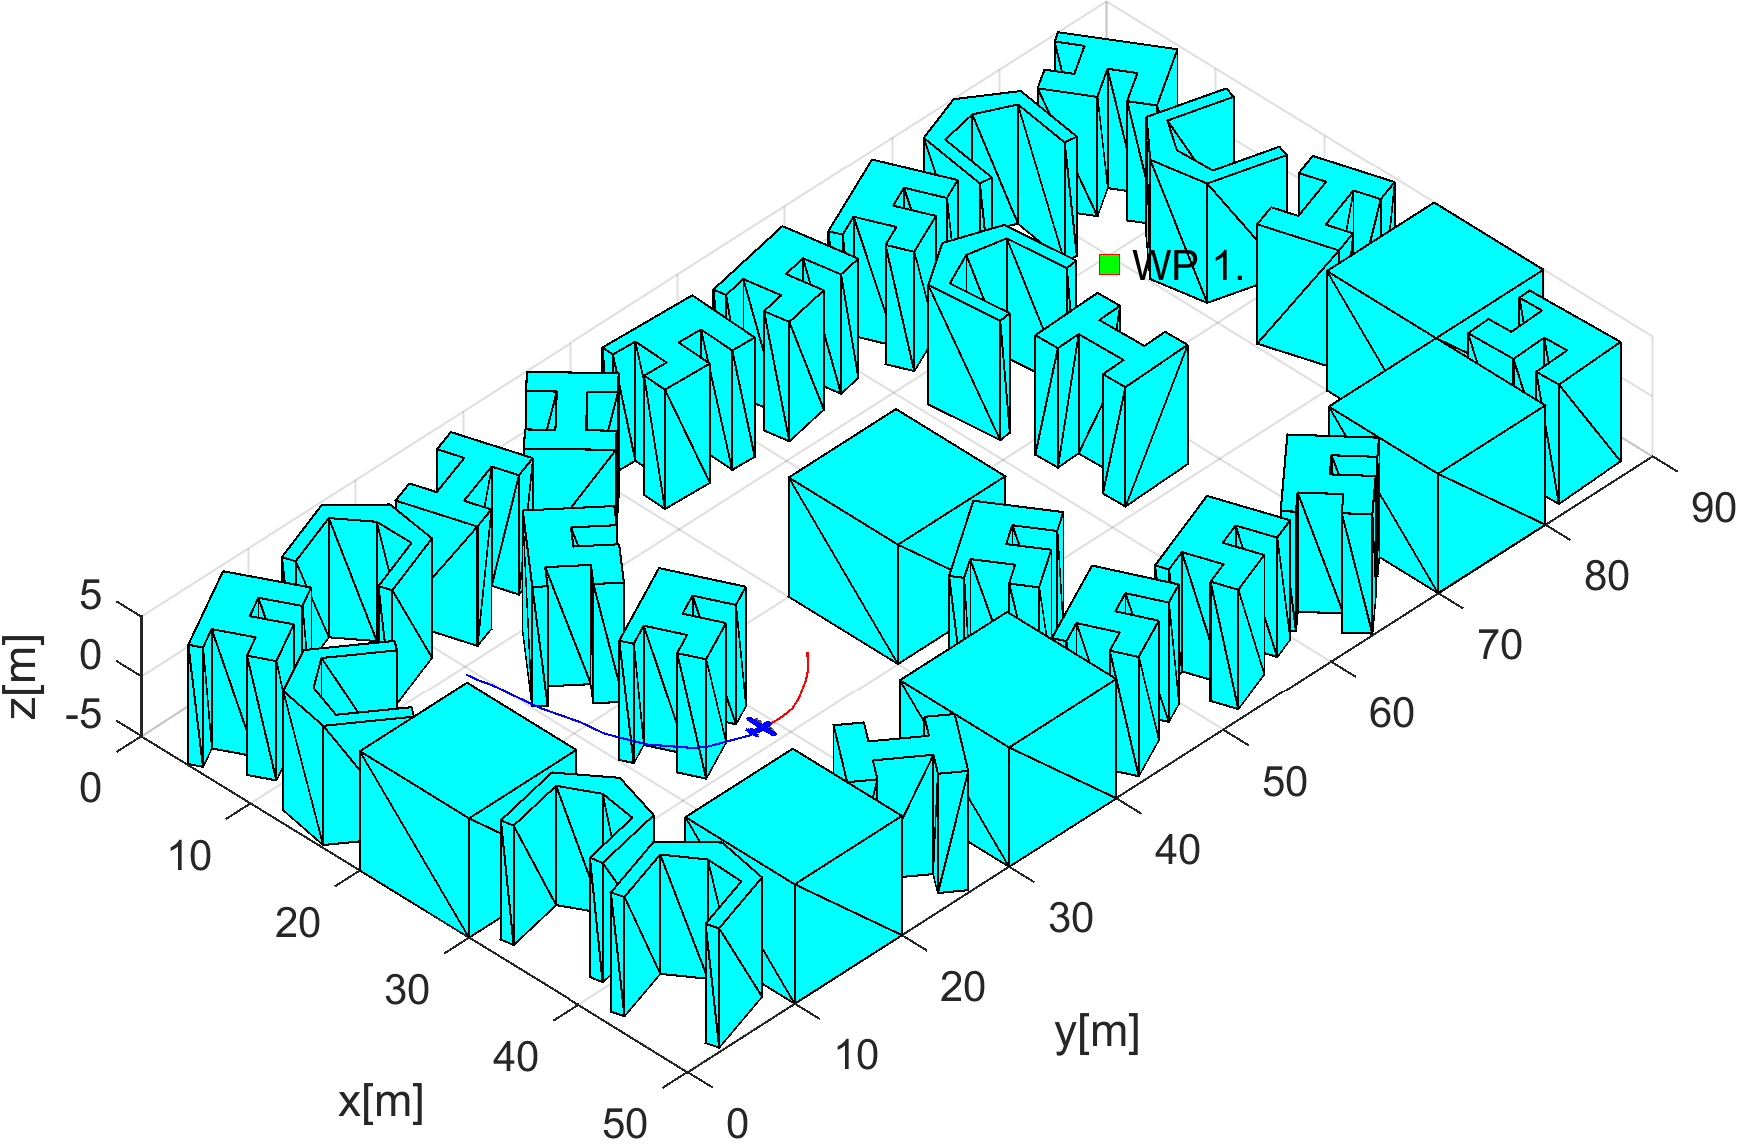
\includegraphics[width=0.9\linewidth]{\FIGDIR/NS013ConstraintsPolynomialMaze00022}
        \caption{$1^{st}$ turn.}
        \label{fig:mazeFirstTurn}
    \end{subfigure}
    \begin{subfigure}{0.48\textwidth}
	    \centering
        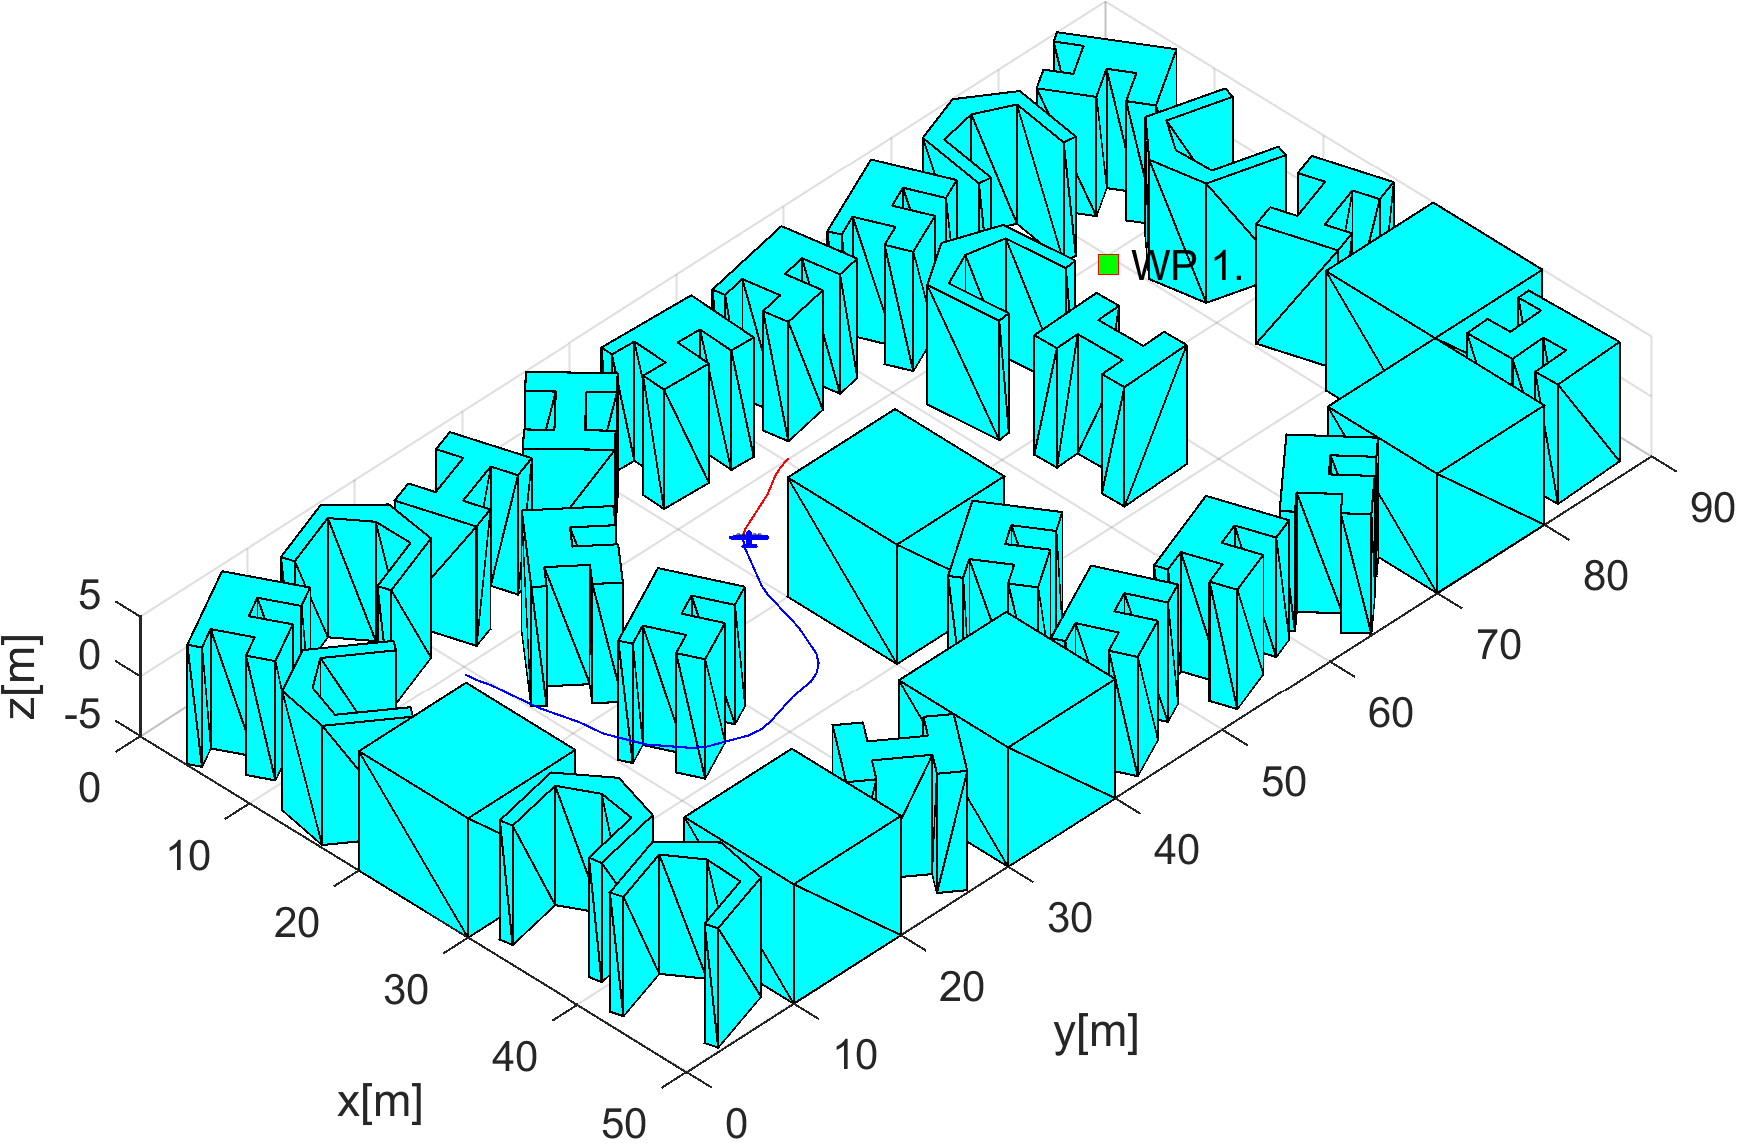
\includegraphics[width=0.9\linewidth]{\FIGDIR/NS014ConstraintsPolynomialMaze00044} 
        \caption{$2^{nd}$ turn.}
        \label{fig:mazeSecondTurn}
    \end{subfigure}
    \\
    \begin{subfigure}{0.48\textwidth}
    	\centering
        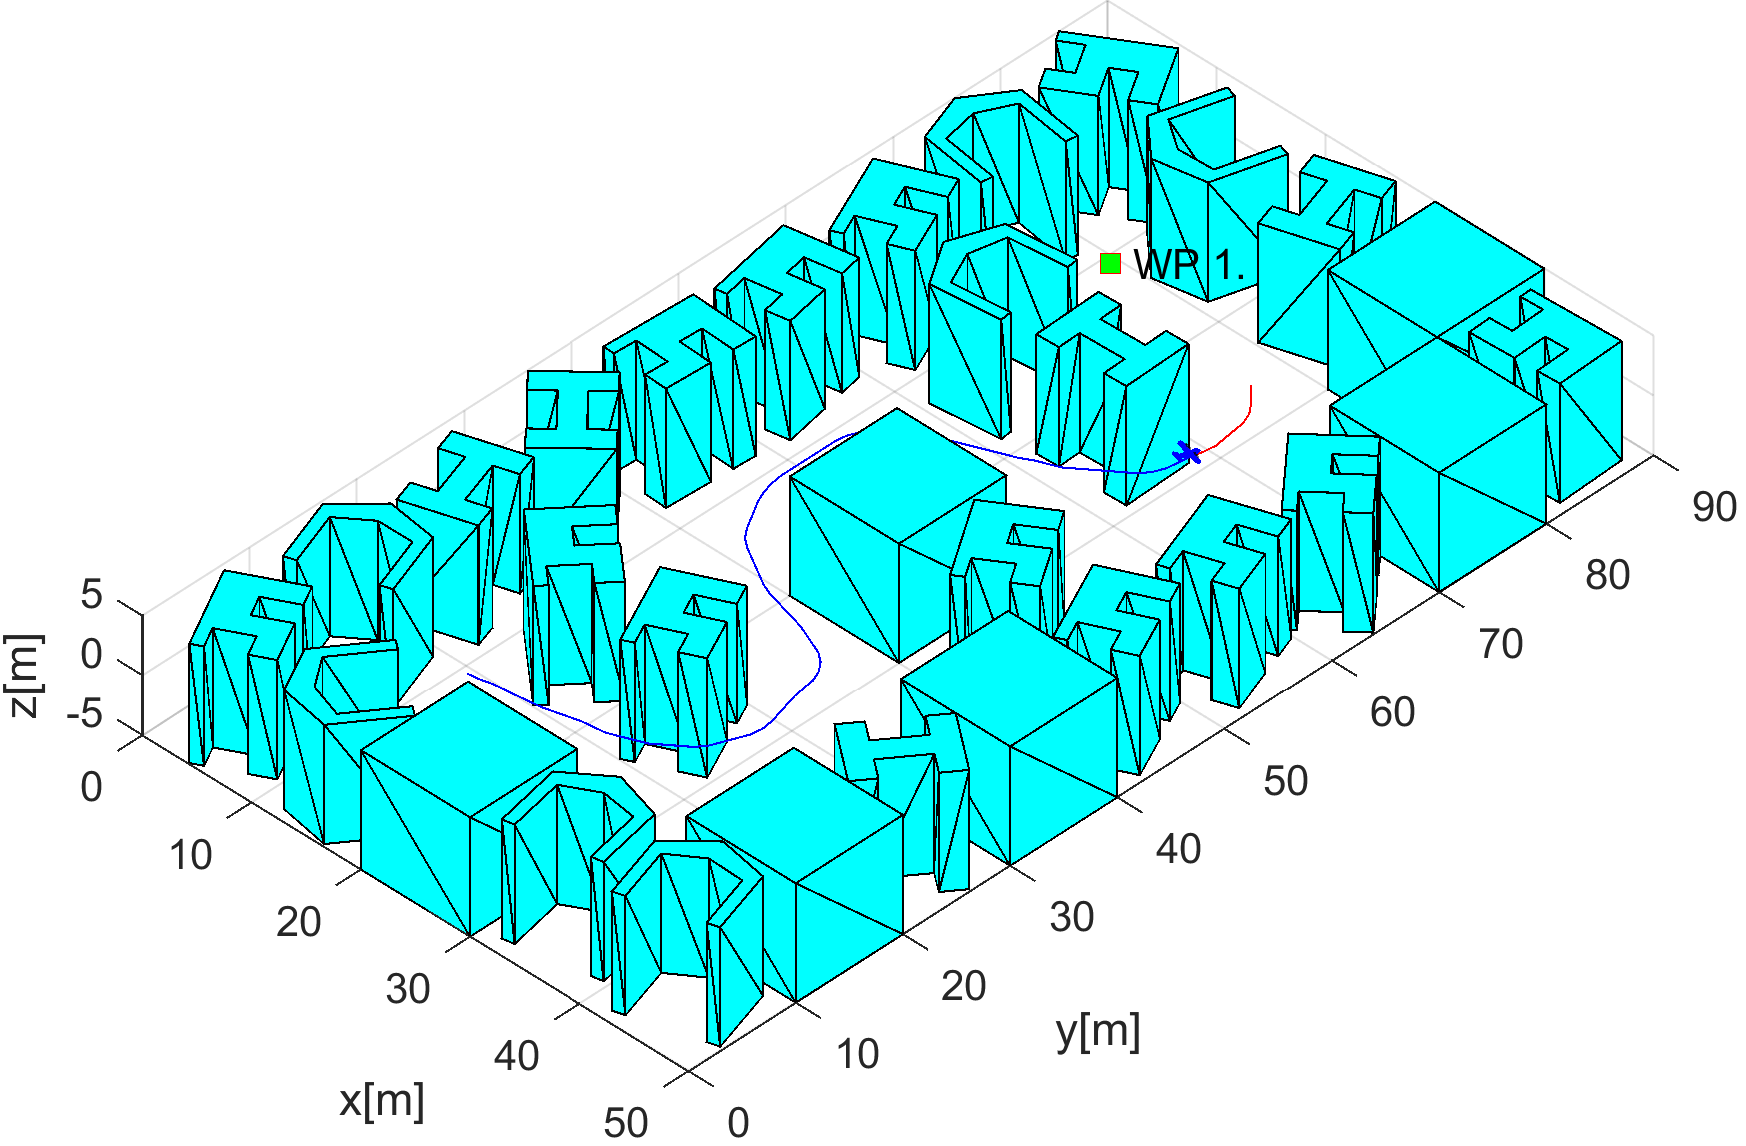
\includegraphics[width=0.9\linewidth]{\FIGDIR/NS015ConstraintsPolynomialMaze00081} 
        \caption{$3^{rd}$ turn.}
        \label{fig:mazeThirdTurn}
    \end{subfigure}
    \begin{subfigure}{0.48\textwidth}
    	\centering
        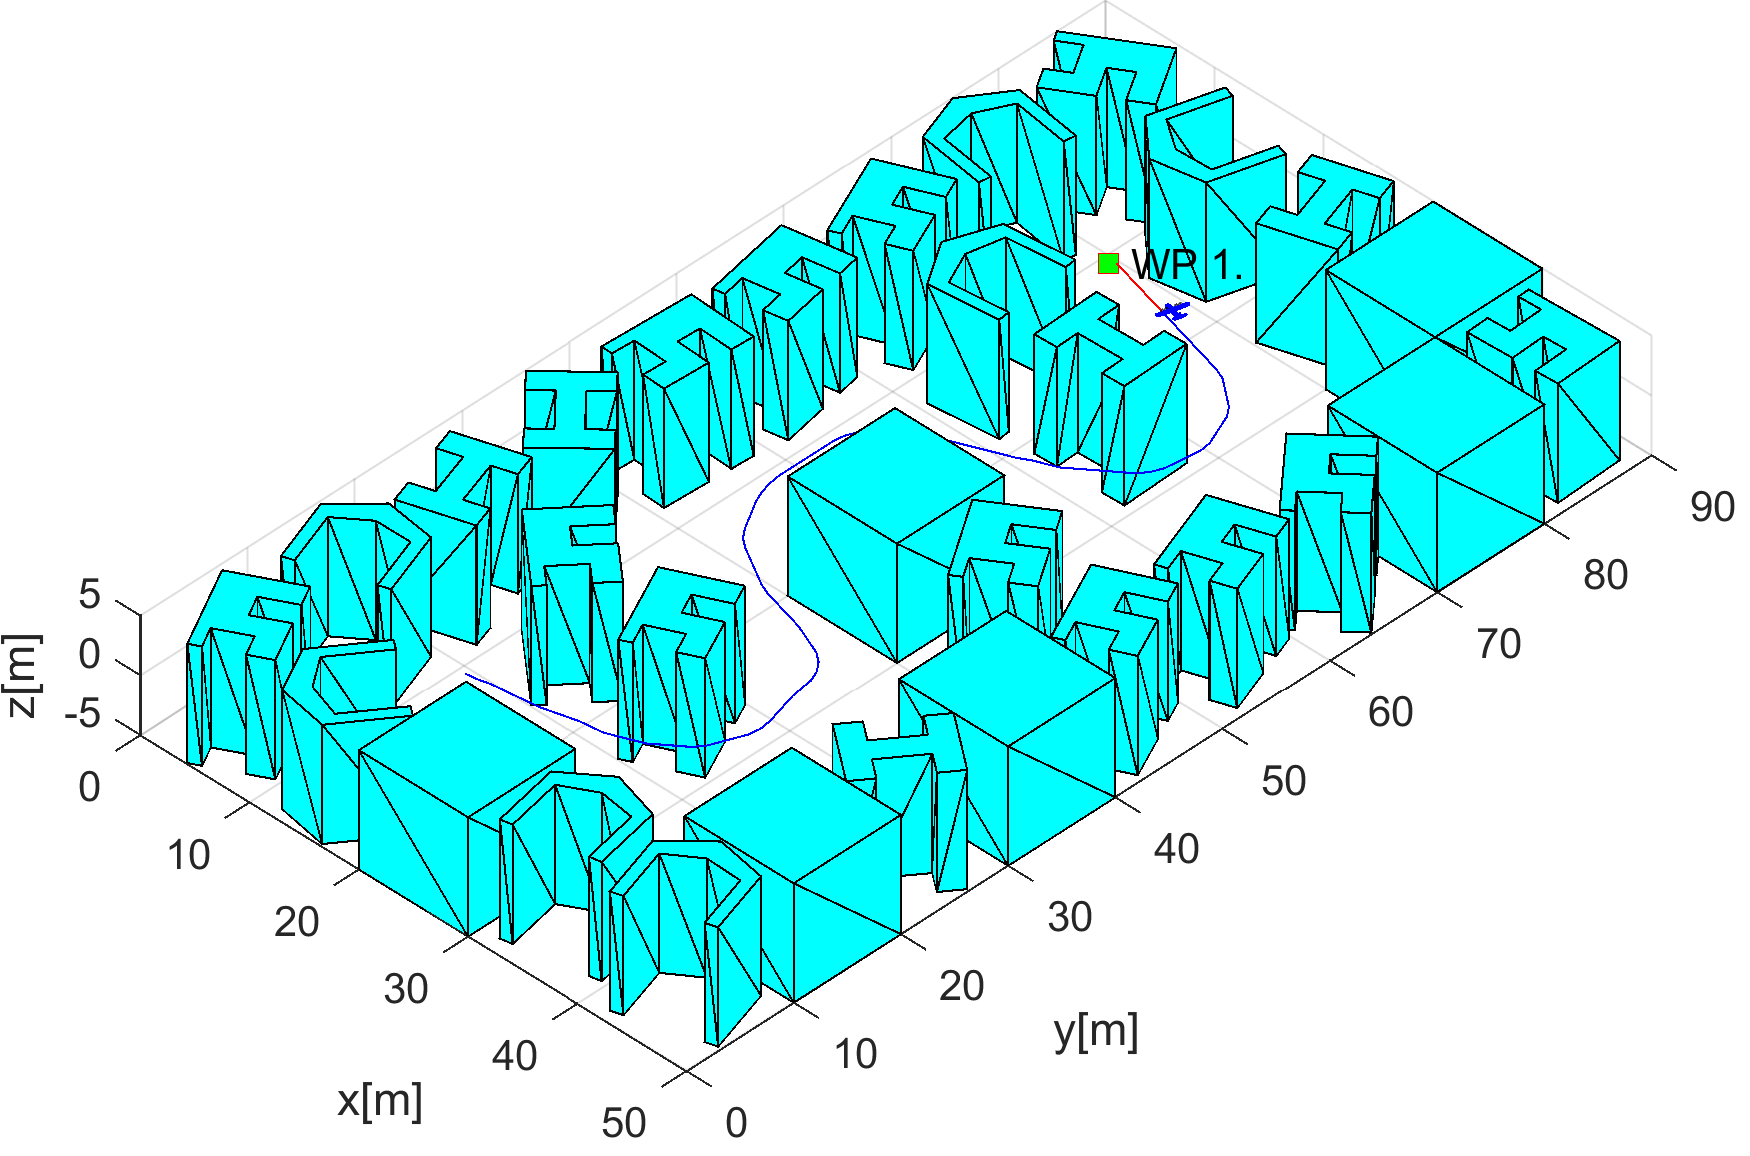
\includegraphics[width=0.9\linewidth]{\FIGDIR/NS016ConstraintsPolynomialMaze00098} 
        \caption{Waypoint reach.}
        \label{fig:mazeWaypointReach}
    \end{subfigure}
    \caption{Test scenario for \emph{Maze}. }
    \label{fig:testCaseMazeSolver}
\end{figure}

\paragraph{Safety Margin Performance:}  The \emph{safety margin performance} over time (x-axis, sec) given in  meters distance (y-axis, m) is given in (fig. \ref{fig:testCaseMazeAvoidancePerformance}).

The \emph{UAS} center distance to nearest obstacle (blue line) does not break any \emph{Safety Margin} (yellow line) of closest obstacle. \emph{Body Margin} of closest obstacle (red line) has not been break, because it always lies below of \emph{Safety Margin} (yellow).

For \emph{UTM time period} $37$ to $68$ sec there is a \emph{margin spike}  due avoidance of bloated \emph{Rectangle buildings} (fig. \ref{fig:mazeSecondTurn}) during $2^{nd}$ turn. The \emph{acceptance criterion} for \emph{Safety Margin} is satisfied.

\begin{note}
The \emph{body} and \emph{safety margin} are changing  depending on \emph{UAS position} and \emph{orientation}. The changes are reflected in (tab. \ref{tab:testCaseMazeSafetyAndBodyMarginDistances}).
\end{note}


\begin{figure}[H]
    \centering
    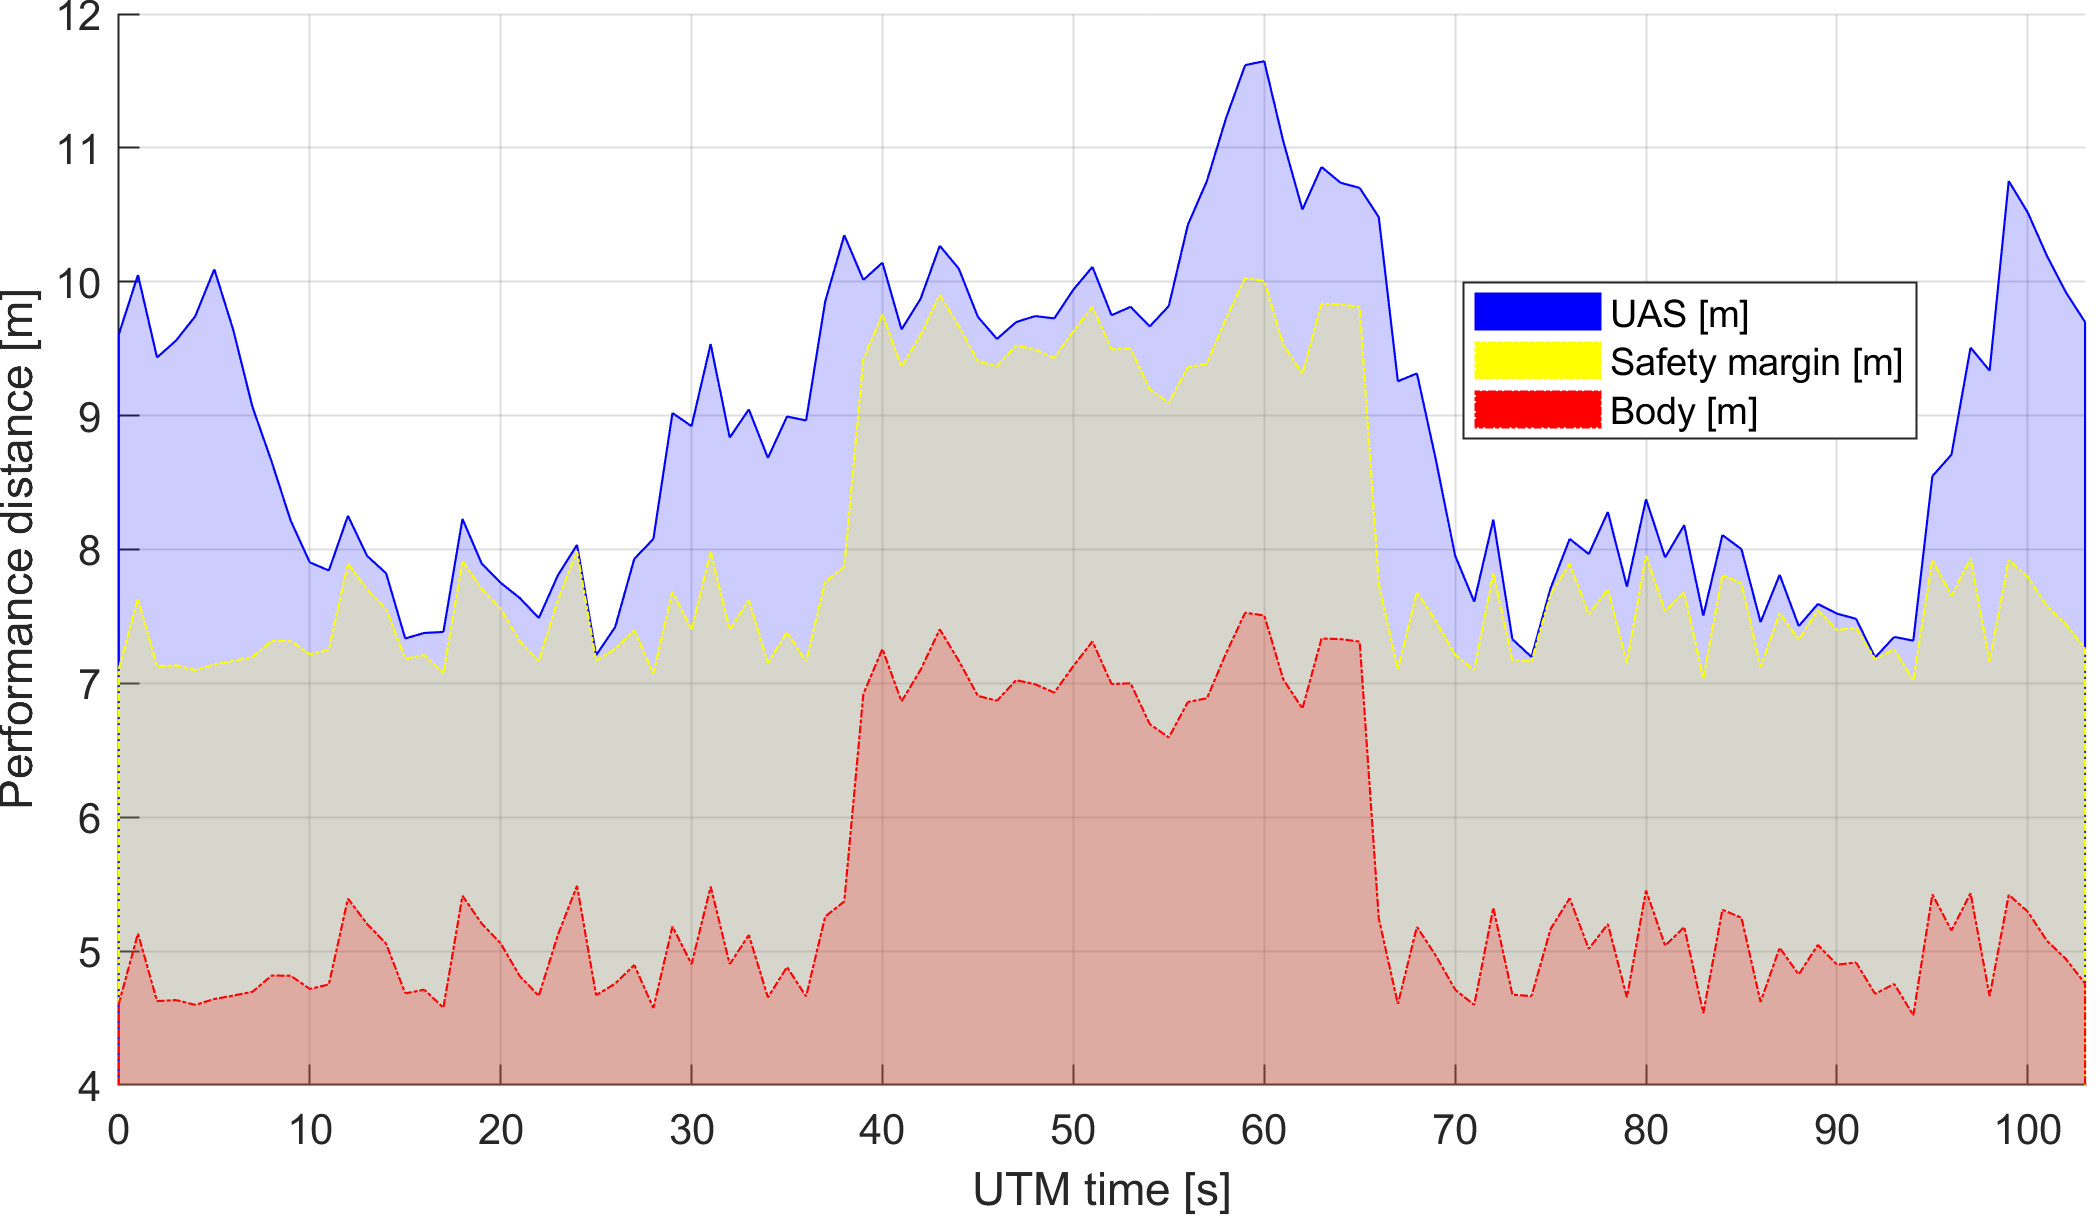
\includegraphics[width=0.8\linewidth]{\FIGDIR/NS017ConstraintsPolynomialMazePerformance} 
    \caption{\emph{Maze} safety margin performance.}
    \label{fig:testCaseMazeAvoidancePerformance}
\end{figure}

\paragraph{Safety Margin distances:} The minimal and maximal values for \emph{UAS body closest point} to \emph{safety margin} distance based on performance (fig. \ref{fig:testCaseMazeAvoidancePerformance}) is summarized in (tab. \ref{tab:testCaseMazeSafetyAndBodyMarginDistances}).

The \emph{minimal distance to safety margin} is $0.0131 m$ which can be taken as $\sim 0m$ due the numerical error. The \emph{maximal distance to safety margin} is $2.9513 m$ which is $5 \times$ \emph{UAS radius}. The safety margin distance is $\le 3 m$ which means the scenario is tightly packed with obstacles. The \emph{UAS} never left \emph{Emergency Avoidance Mode} because condition: $safety Margin Distance \ge avoidance Grid Length$ was never satisfied. 

The \emph{minimal body} distance is $5.0131 m$, while the \emph{maximal body} distance is $8.7117 m$. The difference between minimal and maximal body distance is $\sim 4 m$ which also indicates obstacle packed scenario. 

\begin{table}[H]
    \centering
    \begin{tabular}{c|c||c}
    \multicolumn{2}{c||}{Parameter} & UAS 1 \\\hline\hline
    \multirow{2}{*}{safety margin distance} & min & 0.0131 \\\cline{2-3}
                                            & max & 2.9513 \\\hline
    \multirow{2}{*}{body margin distance}   & min & 5.0131 \\\cline{2-3}
                                            & max & 8.7117 
    \end{tabular}
    \caption{\emph{Maze} safety and body margin distances.}
    \label{tab:testCaseMazeSafetyAndBodyMarginDistances}
\end{table}

\paragraph{Path Tracking Performance:} Reference path (green dashed) line is given as direct interconnection of \emph{initial position} (green square with S marker) and \emph{hidden waypoint} (green square with 1 marker). The \emph{UTM Reference Time} is given on x-axis. The evolution of real trajectory (blue solid line) for each axis is given as follow:

\begin{enumerate}
    \item \emph{X-axis path tracking} - reflects the maneuvering in the curves of the maze.
    
    \item \emph{Y-axis path tracking} - shows horizontal progress to the \emph{hidden goal waypoint}. The expected linear tracking is not achievement due the manuevering delays on X-axis.
    
    \item \emph{Z-axis path tracking} - shows perfect linear tracking of reference trajectory. The \emph{altitude acceptance criterion}: $-5m \le altitude \le 5m$ have been fulfilled.
\end{enumerate}

\begin{figure}[H]
    \centering
    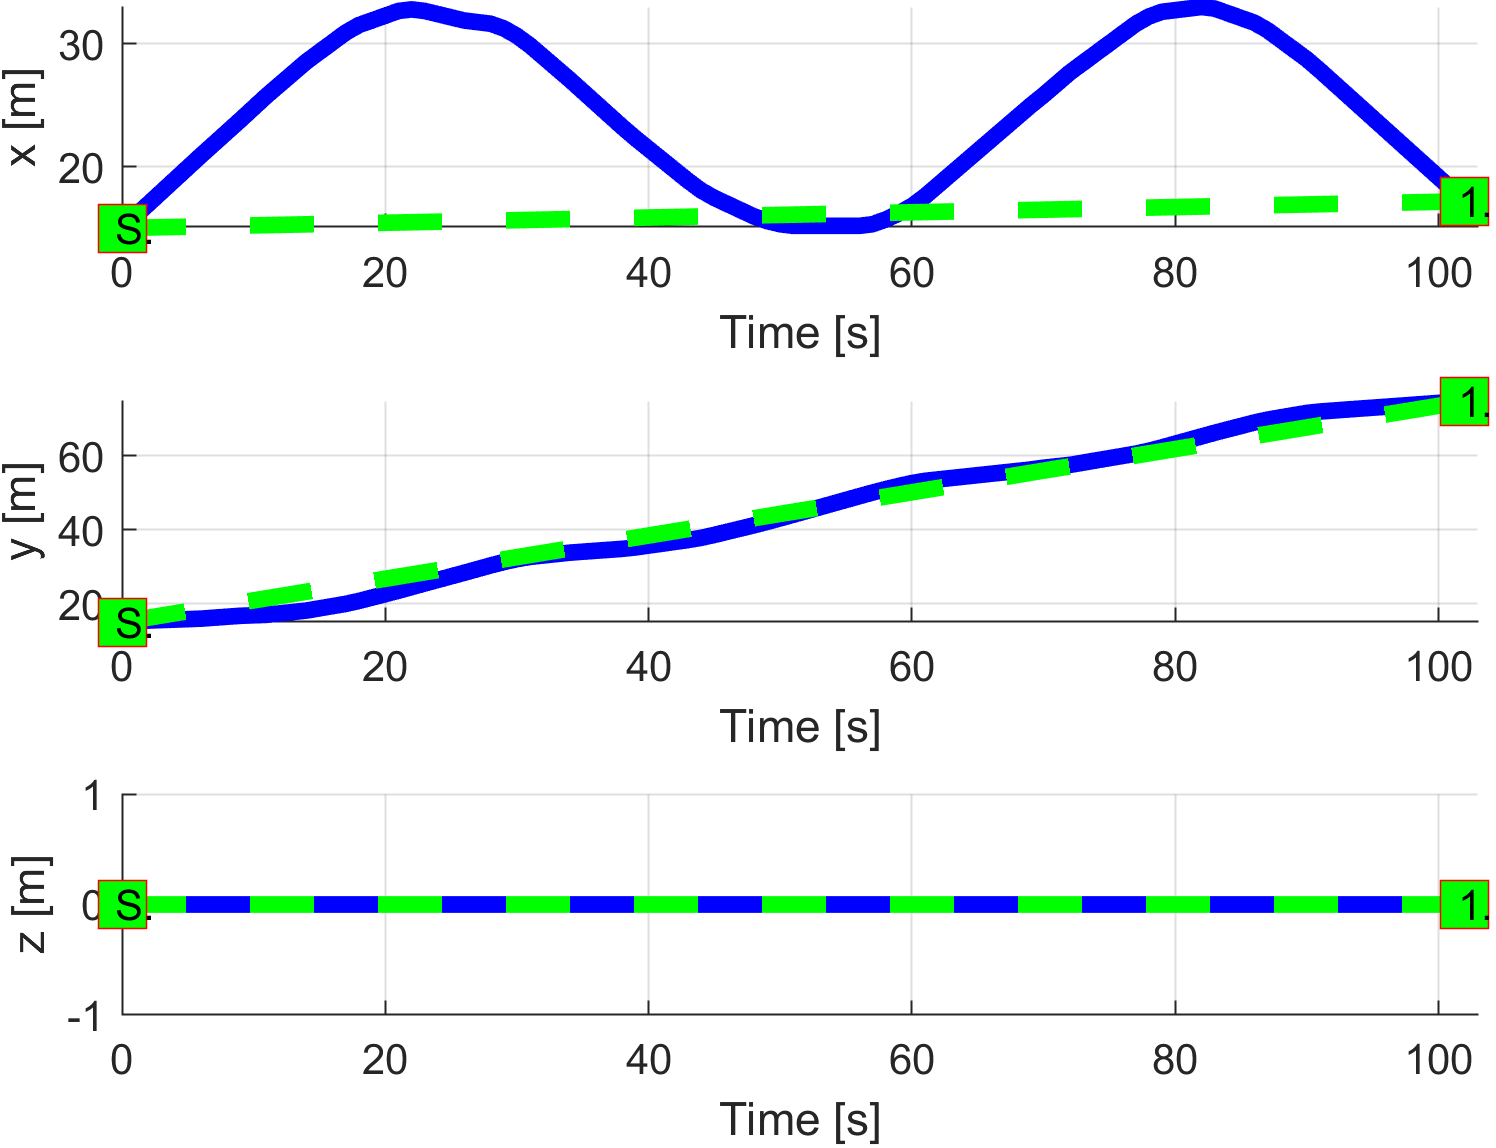
\includegraphics[width=0.55\linewidth]{\FIGDIR/NS018ConstraintsPolynomialMazePathFollowing} 
    \caption{\emph{Maze} path tracking.}
    \label{fig:testCaseMazePathTracking}
\end{figure}


\paragraph{Path Tracking Deviations:} Deviations (tab. \ref{tab:pathTrackingParametersForMazeAvoidance}) from \emph{reference trajectory} are in expected ranges considering \emph{mission plan} (tab. \ref{tab:missionSetupMazeScenario}) and \emph{obstacle properties} (tab. \ref{tab:obstacleSetMaze}).

\begin{table}[H]
    \centering
    \begin{tabular}{c||c}
        \multirow{2}{*}{Param.} & UAS 1\\\cline{2-2}
                        & $\mathscr{WP}_1$  \\\hline\hline
          $\max |x|$    & 27.32             \\\hline
          $\max |y|$    & 2.41             \\\hline
          $\max |z|$    & 0                 \\\hline
          $\max dist.$  & 28.06             \\
    \end{tabular}
    \caption{Path tracking properties for \emph{Maze} scenario.}
    \label{tab:pathTrackingParametersForMazeAvoidance}
\end{table}


